% A sealed box of hot gas cut by an imaginary plane. Forces on each half across
% the cut: the gas pushes the halves apart; the walls, under tension, pull them
% together. Equilibrium: the two balance for every cut.
\documentclass[tikz,border=1pt]{standalone}
% Shared preamble for the standalone figures: the book's fonts, palette and
% drawing styles. Figures are drawn at their final printed size. A column is
% 3.35in (241pt) wide; a figure across both columns is 7in (505pt) wide.

\usepackage[T1]{fontenc}
\usepackage{newpxtext}
\usepackage[varbb]{newpxmath}
\usepackage[semibold,scale=0.95,lining]{sourcesanspro}
\usepackage{xcolor}
% Palette shared by the book and by the standalone figures in figures/src.
% One main hue (blue), one accent (orange), and a few roles used sparingly.

\definecolor{seblue}{HTML}{1D5B8F}    % headings, worked examples, main curves
\definecolor{seblueDark}{HTML}{123E63}
\definecolor{seorange}{HTML}{DC7A26}  % thought experiments, light and light cones
\definecolor{seteal}{HTML}{1F8577}    % checks, travellers and ships
\definecolor{sered}{HTML}{C0392B}     % negative energy, tension, violations
\definecolor{seviolet}{HTML}{5E548E}  % going deeper
\definecolor{sesand}{HTML}{8C6A3F}    % history
\definecolor{segray}{HTML}{6B7480}    % axes, guides, secondary labels
\definecolor{selight}{HTML}{D5DAE1}   % grids and faint rules

\usepackage{siunitx}
\usepackage{fontawesome5}
\usepackage{tikz}
\usetikzlibrary{arrows.meta,calc,positioning,decorations.pathreplacing,
  decorations.markings,shapes.geometric,fadings,shadings,patterns,3d,
  intersections,backgrounds}
\usepackage{pgfplots}
\pgfplotsset{compat=1.18}
\usepgfplotslibrary{fillbetween,groupplots,colormaps}

\tikzset{
  >={Latex[length=2.1mm,width=1.4mm]},
  every picture/.style={line cap=round, line join=round},
  lbl/.style={font=\sffamily\footnotesize, text=black!85},
  smalllbl/.style={font=\sffamily\scriptsize, text=black!75},
  guide/.style={segray, line width=0.4pt},
  axisline/.style={segray, line width=0.5pt, -{Latex[length=1.7mm,width=1.1mm]}},
  light/.style={seorange, line width=0.9pt},
  lightdash/.style={seorange, line width=0.9pt, dash pattern=on 3pt off 2pt},
  ship/.style={seteal, line width=1.4pt},
  cone/.style={fill=seorange!22, draw=seorange!85!black, line width=0.35pt},
}

\pgfplotsset{
  se axis/.style={
    axis lines=left,
    axis line style={segray, line width=0.5pt, -{Latex[length=1.6mm,width=1.1mm]}},
    tick style={segray, line width=0.4pt},
    major tick length=2.5pt,
    tick label style={font=\sffamily\scriptsize, text=black!75},
    label style={font=\sffamily\footnotesize, text=black!85},
    every axis plot/.append style={line width=1.1pt},
    legend style={font=\sffamily\scriptsize, draw=none, fill=none},
    scaled ticks=false,
    xticklabel={\sansnum{\tick}}, yticklabel={\sansnum{\tick}},
  },
}

% Numbers in figures are set in the sans-serif text font, with a true minus.
\sisetup{mode=text, reset-text-family=false, reset-text-series=false,
  reset-text-shape=false, drop-zero-decimal, group-minimum-digits=5}
% Tick values arrive as long decimals (1.5000000000); parse them first.
\newcommand{\sansnum}[1]{\begingroup\pgfkeys{/pgf/fpu=false}%
  \pgfmathparse{1*(#1)}\num{\pgfmathresult}\endgroup}

\begin{document}
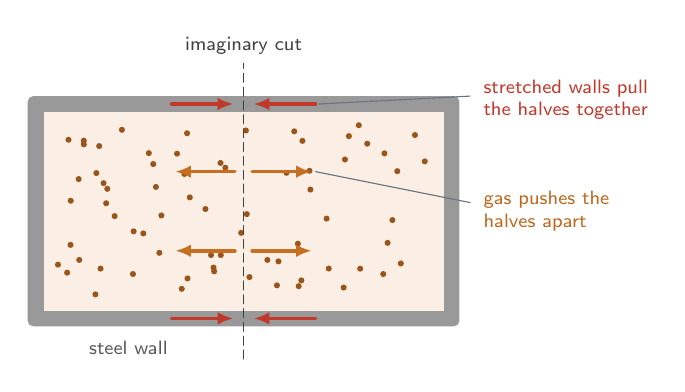
\begin{tikzpicture}[x=26pt, y=26pt]
% walls and gas
\fill[black!40, rounded corners=2pt] (-3,-1.6) rectangle (3,1.6);
\fill[seorange!12] (-2.78,-1.38) rectangle (2.78,1.38);
\pgfmathsetseed{7}
\foreach \k in {1,...,70} {
  \pgfmathsetmacro{\px}{-2.6 + 5.2*rnd}
  \pgfmathsetmacro{\py}{-1.2 + 2.4*rnd}
  \fill[seorange!70!black] (\px,\py) circle (1.1pt);
}
% the cut
\draw[black!75, line width=0.7pt, dash pattern=on 3pt off 2pt] (0,-2.05) -- (0,2.05);
\node[smalllbl, anchor=south] at (0,2.05) {imaginary cut};
% gas pushes the halves apart
\foreach \y in {-0.55,0.55} {
  \draw[seorange!90!black, line width=1.3pt, -{Latex[length=2mm,width=1.6mm]}] (0.12,\y) -- (0.95,\y);
  \draw[seorange!90!black, line width=1.3pt, -{Latex[length=2mm,width=1.6mm]}] (-0.12,\y) -- (-0.95,\y);
}
% walls pull the halves together
\foreach \y in {-1.49,1.49} {
  \draw[sered, line width=1.3pt, -{Latex[length=2mm,width=1.6mm]}] (1.0,\y) -- (0.14,\y);
  \draw[sered, line width=1.3pt, -{Latex[length=2mm,width=1.6mm]}] (-1.0,\y) -- (-0.14,\y);
}
\node[smalllbl, text=seorange!85!black, anchor=west, align=left] at (3.2,0.0)
  {gas pushes the\\halves apart};
\draw[guide] (1.0,0.55) -- (3.15,0.12);
\node[smalllbl, text=sered, anchor=west, align=left] at (3.2,1.55)
  {stretched walls pull\\the halves together};
\draw[guide] (1.05,1.49) -- (3.15,1.6);
\node[smalllbl, text=black!65] at (-1.6,-1.9) {steel wall};
\end{tikzpicture}
\end{document}
